%----------------------------------------------------------------------------------------
%	PACKAGES AND OTHER DOCUMENT CONFIGURATIONS
%----------------------------------------------------------------------------------------

\documentclass[a0,portrait]{a0poster}

\usepackage{multicol} % This is so we can have multiple columns of text side-by-side
\columnsep=100pt % This is the amount of white space between the columns in the poster
\columnseprule=3pt % This is the thickness of the black line between the columns in the poster

\usepackage[svgnames]{xcolor} % Specify colors by their 'svgnames', for a full list of all colors available see here: http://www.latextemplates.com/svgnames-colors

\usepackage{times} % Use the times font
%\usepackage{palatino} % Uncomment to use the Palatino font

\usepackage{graphicx} % Required for including images
\graphicspath{{figures/}} % Location of the graphics files
\usepackage{booktabs} % Top and bottom rules for table
\usepackage[font=small,labelfont=bf]{caption} % Required for specifying captions to tables and figures
\usepackage{amsfonts, amsmath, amsthm, amssymb} % For math fonts, symbols and environments
\usepackage{wrapfig} % Allows wrapping text around tables and figures

\begin{document}

%----------------------------------------------------------------------------------------
%	POSTER HEADER 
%----------------------------------------------------------------------------------------

% The header is divided into two boxes:
% The first is 75% wide and houses the title, subtitle, names, university/organization and contact information
% The second is 25% wide and houses a logo for your university/organization or a photo of you
% The widths of these boxes can be easily edited to accommodate your content as you see fit

\begin{minipage}[b]{0.75\linewidth}
\veryHuge \color{NavyBlue} \textbf{Modeling the Evolution of Mimicry} \color{Black}\\\\ % Title
\huge \textbf{Mohiul Islam \& Peter Grogono}\\[0.5cm] % Author(s)
\huge Engineering \& Computer Science, Concordia University\\[0.4cm] % University/organization
\Large \texttt{moh\_i@encs.concordia.ca \& grogono@cse.concordia.ca}\\
\end{minipage}
%
\begin{minipage}[b]{0.25\linewidth}

\includegraphics[width=20cm]{logo.jpg}\\
\end{minipage}

\vspace{1cm} % A bit of extra whitespace between the header and poster content

%----------------------------------------------------------------------------------------

\begin{multicols}{2} % This is how many columns your poster will be broken into, a portrait poster is generally split into 2 columns

%----------------------------------------------------------------------------------------
%	ABSTRACT
%----------------------------------------------------------------------------------------

\color{Navy} % Navy color for the abstract

\begin{abstract}

A novel agent based, artificial life model, for the evolution of mimicry is presented. This model is a predator-prey co-evolution scenario where pattern representation phenotype is simulated with Cellular Automata (CA), while behaviors of pattern recognition is configured with Hopfield Network. A visual three dimensional toroidal cube is used to construct a universe in which agents have complete freedom of mobility, genetic representation of behavior and reproduction capability to evolve new behaviors in successive generations. These agents are classified into categories of predator and prey species. Genome of prey species control their mobility and palatability, while 2D CA is used to represent a pattern, where the rule to generate the CA is also genetically represented. Through evolution, successive generations of prey species develop new patterns to represent them both visually and to the predators. Predators are agents with the primary purpose of providing selection pressure for the evolution of mimicry. They are equipped with Hopfield Network memory to recognize new CA pattern and make intelligent decisions to consume the prey based on their level of palatability. Using the above construction of ideas, successful emulation of the natural process of mimicry is achieved. Also complex behavior pattern of Batesian and Mullerian mimicry is simulated and studied.

\end{abstract}

%----------------------------------------------------------------------------------------
%	INTRODUCTION
%----------------------------------------------------------------------------------------

\color{SaddleBrown} % SaddleBrown color for the introduction

\section*{Introduction}

Mimicry is a process of deception. It is an evolutionary process with the help of which organisms survive by deceiving its predator. But this deception happens only if the environment contains similar appearing noxious organisms which the predators find unpalatable. Palatable organisms mimic the unpalatable ones through the process of evolution for survival of its species. The objective of this paper is to present an agent based artificial life model for simulating this natural process of the evolution of mimicry.

\color{DarkSlateGray} % DarkSlateGray color for the rest of the content

%----------------------------------------------------------------------------------------
%	The Inspiration: Mimicry
%----------------------------------------------------------------------------------------

\section*{The Inspiration: Mimicry}
\subsection*{Batesian Mimicry}
Henry W. Bates first published in 1862 his findings about the similarities and dissimilarities between Heliconiinae and Ithomiinae butterflies. He found butterflies having similar appearance, exhibiting morphological features which point to completely different species even families. Even though Heliconiids are conspicuously colored, they are extremely abundant. They are also slow in mobility. Still predators in the surrounding area, mostly insectivorous birds do not prey on them, because of their inedible and unpalatable nature. Other edible and palatable species such as ithomiinae and pieridae, pretend to be heliconiids and thus enjoy protection. In general, the animal which is avoided by predator for unpalatable behavior is called the \textbf{model} and the imitating animal is called the \textbf{mimic}.

\begin{center}\vspace{1cm}
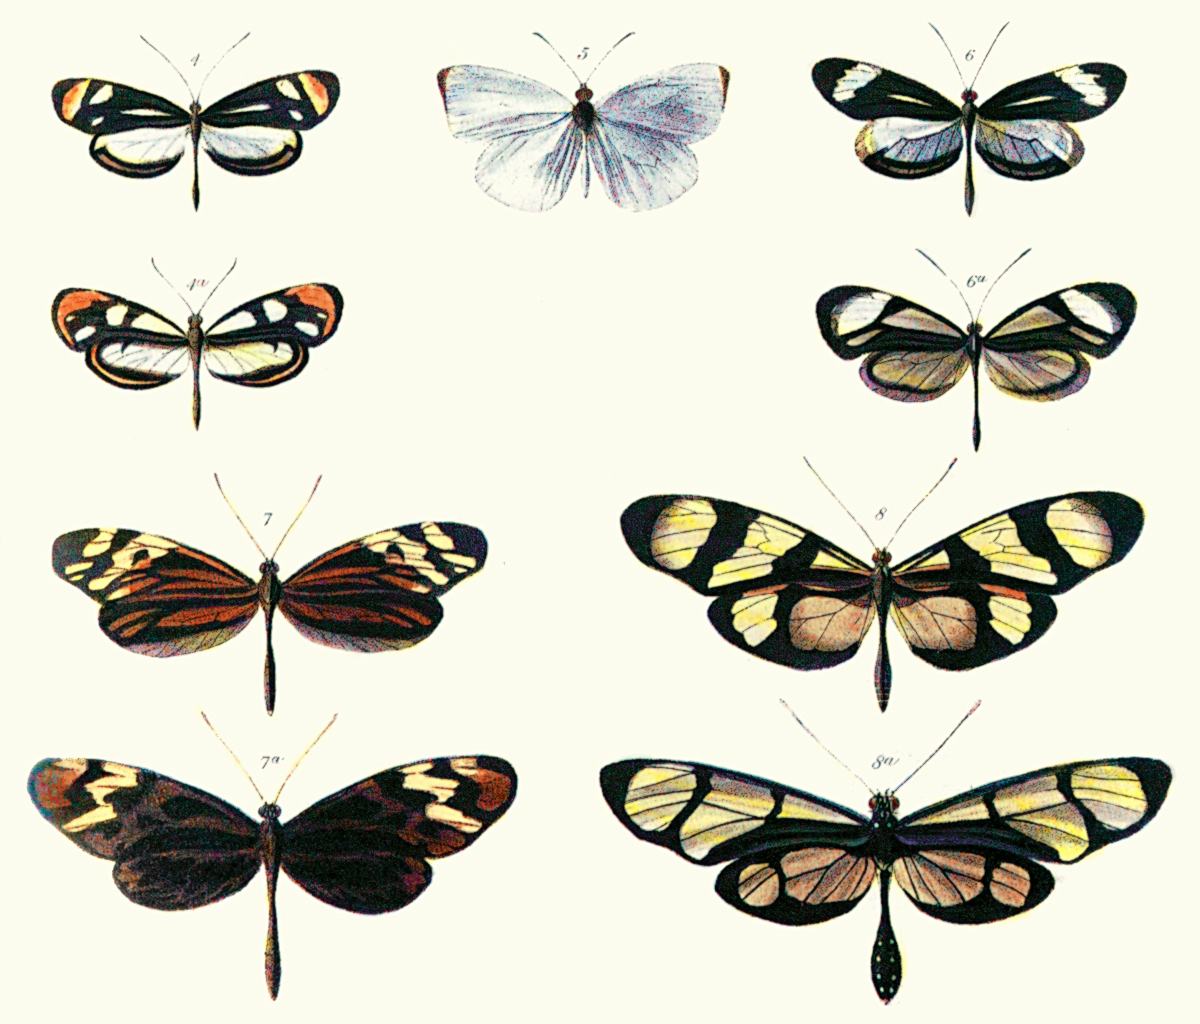
\includegraphics[width=0.5\linewidth]{Batesplate_ArM.jpg}
\captionof{figure}{\color{Green} Plate from Bates (1862) illustrating Batesian mimicry between Dismorphia species (top row, third row) and various Ithomiini (Nymphalidae) (second row, bottom row)}
\end{center}\vspace{1cm}

\subsection*{Mullerian Mimicry}
Bates was not able to explain some phenomena of mimicry. Occasionally two inedible unrelated butterfly species are amazingly similar in appearance. An explanation for this was provided by Fritz Muller in 1878. When there are multiple inedible species it is hard for predators to recognize each of them to know which one to consume and which one to avoid. Because of the predator's limited memory, all these species still lose their number even after being inedible. So to save this loss, and to prevent more sacrifice of their own kind, inedible species from different families also tend to evolve to have similar appearance. This phenomena is referred to as Mullerian Mimicry in the name of Fritz Muller. Like Batesian mimicry, Mullerian mimicry can evolve in two stages: the mutational, one way convergence stage followed by the gradual, mutual convergence stage.

\section*{The Model: Evolution of Mimicry}

Our model initializes with three kinds of agents. These agents have properties and behavior similar to the \textbf{model}, the \textbf{mimic} and the \textbf{predator}. We represent evolution of pattern for the model and the mimic with the help of \textbf{CA}, as \textbf{CA} can be easily represented by simple rules. Each predator is equipped with a Hopfield network, which gives it pattern recognition capability. The process of evolution occurs at the genetic level. 

\begin{center}\vspace{1cm}
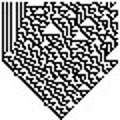
\includegraphics[width=0.1\linewidth]{CARule30-large.jpg}
\captionof{figure}{\color{Green} Cellular Automata Rule 30}
\end{center}\vspace{1cm}

This model has been designed to come up with efficient results and achieve the main objective, \textit{evolution of mimicry}. Creation and transformation of different mimicry ring and also the dynamics of it has been integrated to achieve interesting results. This model can also be considered as a complex adaptive system similar to Holland's work on Echo.

\begin{center}\vspace{1cm}
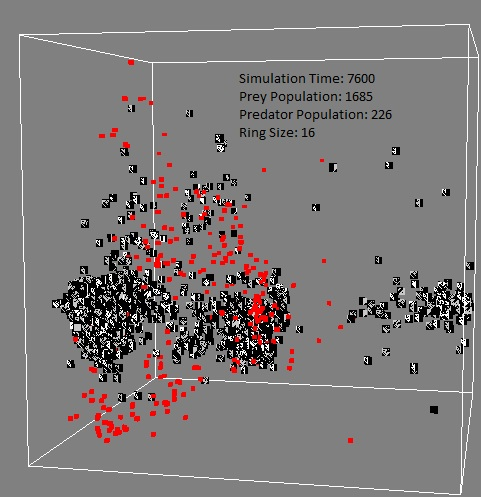
\includegraphics[width=0.5\linewidth]{simTime7600.jpg}
\captionof{figure}{\color{Green} Graphical representation of the model, simulation time: 7600}
\end{center}\vspace{1cm}

\section*{The Results}

Data and analysis in this simulation has been concentrated on evaluating whether evolution of mimicry has taken place. This evaluation can be made with the number of different rings that has been created and the size of each of those rings along with the population of palatable and unpalatable species. Also it can be established whether Batesian Mimicry and Mullerian Mimicry have taken effect by analyzing the data set of these populations.

\subsection*{Initial configuration with two prey species}

\begin{center}\vspace{1cm}
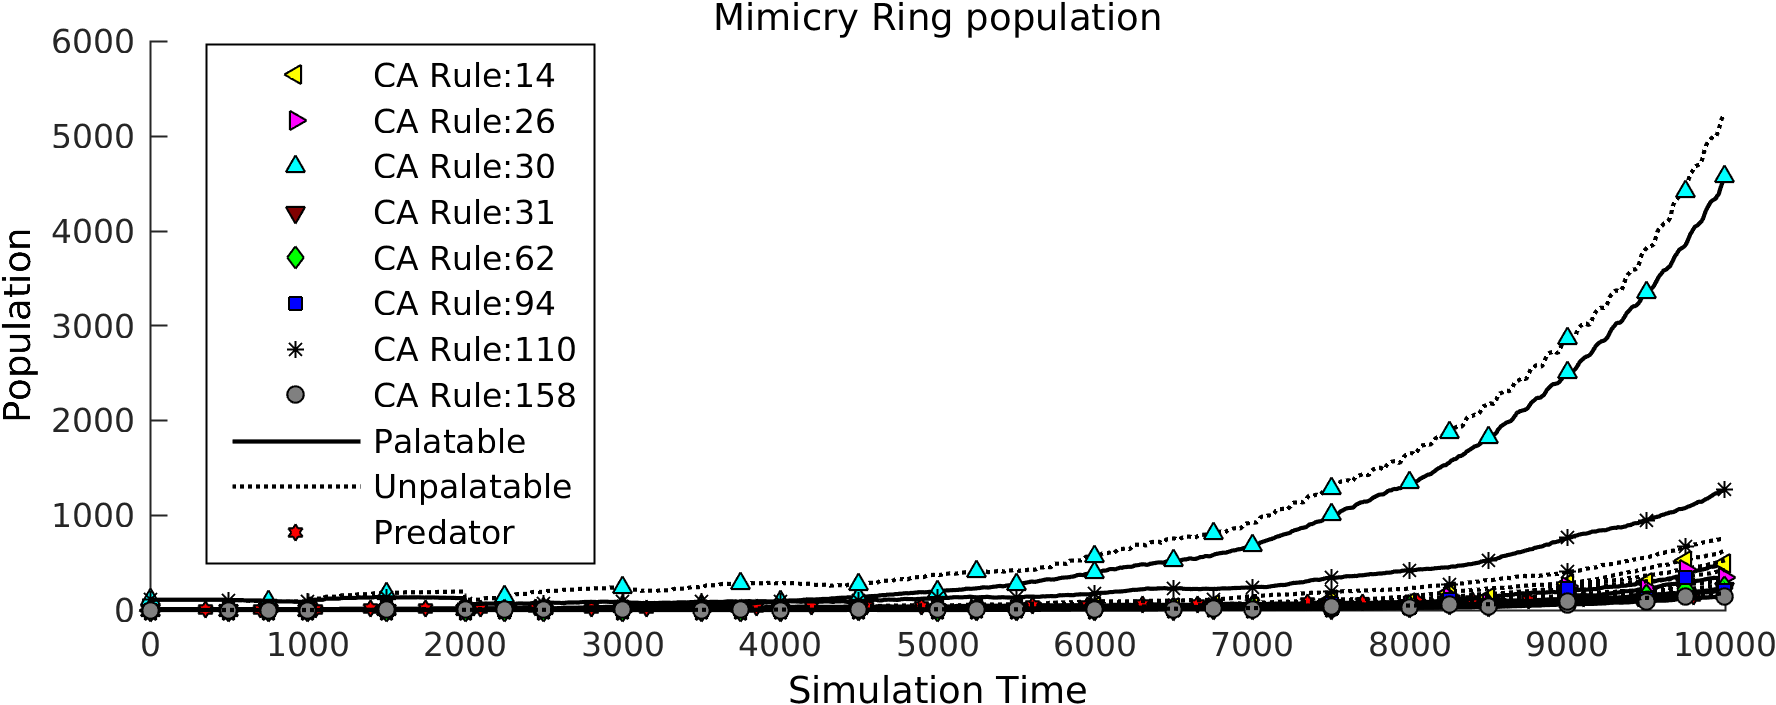
\includegraphics[width=0.8\linewidth]{simTime10k-2Prey.png}
\captionof{figure}{\color{Green} Population distribution of mimicry rings, initialized with 2 prey species, 10k iterations}
\end{center}\vspace{1cm}

\subsection*{Initial configuration with only unpalatable species}

\begin{center}\vspace{1cm}
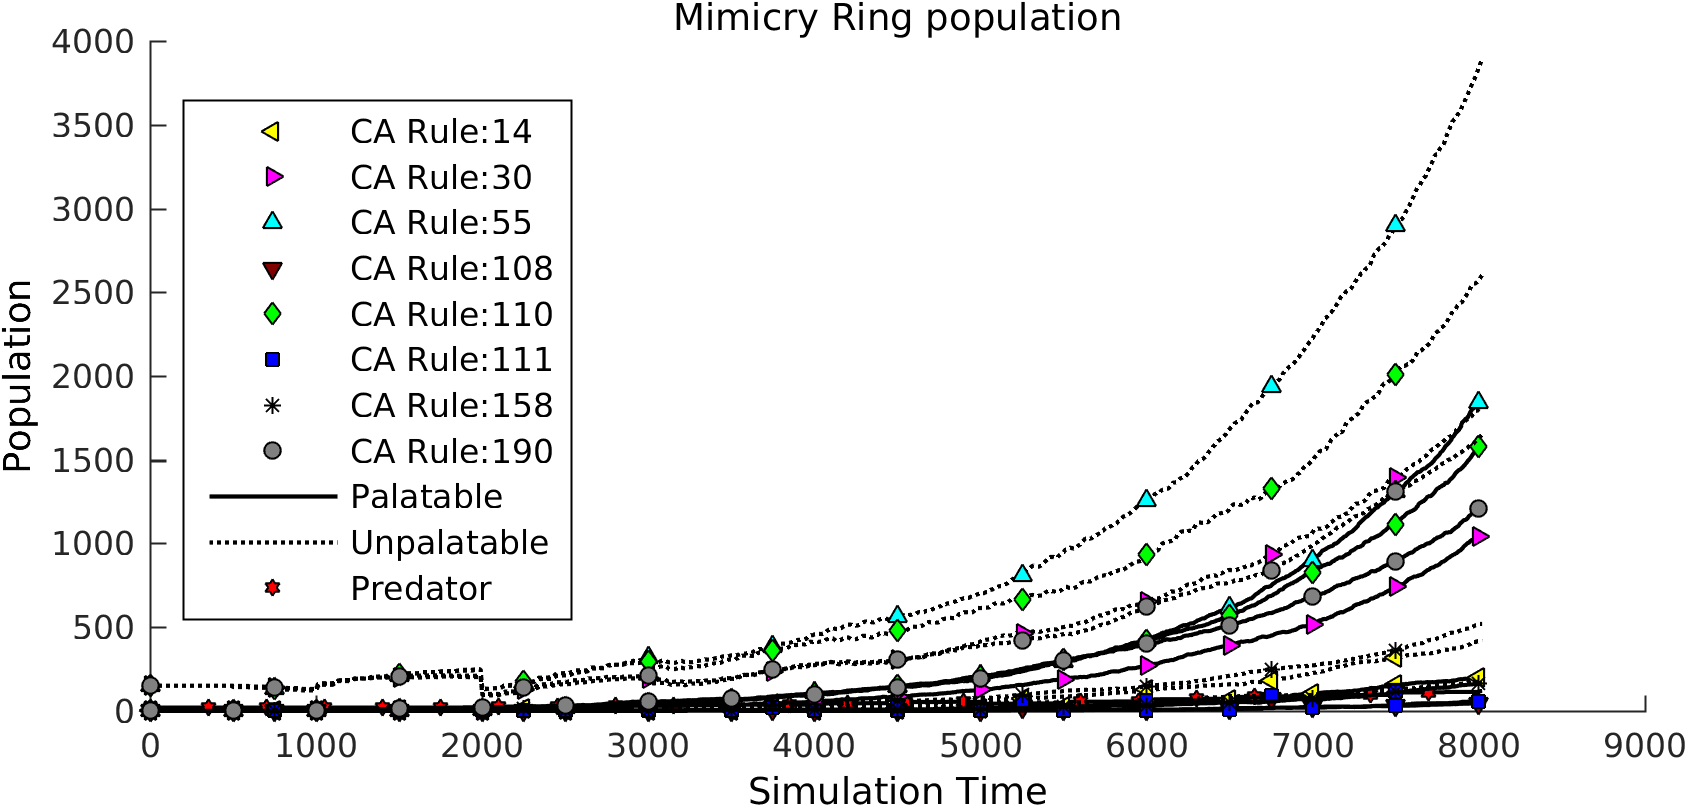
\includegraphics[width=0.8\linewidth]{simTime8k-4Prey-unp.png}
\captionof{figure}{\color{Green} Population distribution of mimicry rings, initialized with 4 prey species all unpalatable}
\end{center}\vspace{1cm}

\subsection*{Analysis}
\begin{itemize}
\item Batesian mimicry has taken effect as it can be observed that for every ring of unpalatable species there is an existence of the palatable ring racing to reach the population count of its unpalatable counterpart.
\item Effects of Mullerian mimicry can also be observed best for the experiment initialized with only unpalatable prey species. We initialized the model with 4 rings of unpalatable species with no palatable ones and after nearly 10K iterations, all of the initial unpalatable rings have survived with dominance. 
\end{itemize}
%----------------------------------------------------------------------------------------
%	CONCLUSIONS
%----------------------------------------------------------------------------------------

\color{SaddleBrown} % SaddleBrown color for the conclusions to make them stand out

\section*{Conclusions}
\begin{itemize}
\item Analysis of the results tell us that we have successfully been able to simulate the evolution of mimicry.
\item This model provides a more accurate simulation of the fascinating natural process of mimicry rings and their shift in population. 
\item This model also verifies the theory of Turner in explaining the evolution of mimicry with punctuated equilibrium.
\end{itemize}

\color{DarkSlateGray} % Set the color back to DarkSlateGray for the rest of the content

%----------------------------------------------------------------------------------------
%	REFERENCES
%----------------------------------------------------------------------------------------

\nocite{*} % Print all references regardless of whether they were cited in the poster or not
\bibliographystyle{plain} % Plain referencing style
\bibliography{sample} % Use the example bibliography file sample.bib

%----------------------------------------------------------------------------------------

\end{multicols}
\end{document}